\chapter{Model Validations}
\label{validation}

\section{Validation of One-Stage Experiment Results}

After identifying the paramaters for all the required equation, developed algorithm model now was built to estimate the contact force. Hence, there are two versions of algortithm, one that use Dahl and another one that use coulomb and viscous. The estimated force is then compared to real force from F/T sensor for validation. The results are shown in \fref{fig:validation}.

\begin{figure}[H]
  \begin{subfigure}[t]{0.5\textwidth}
    \centering
    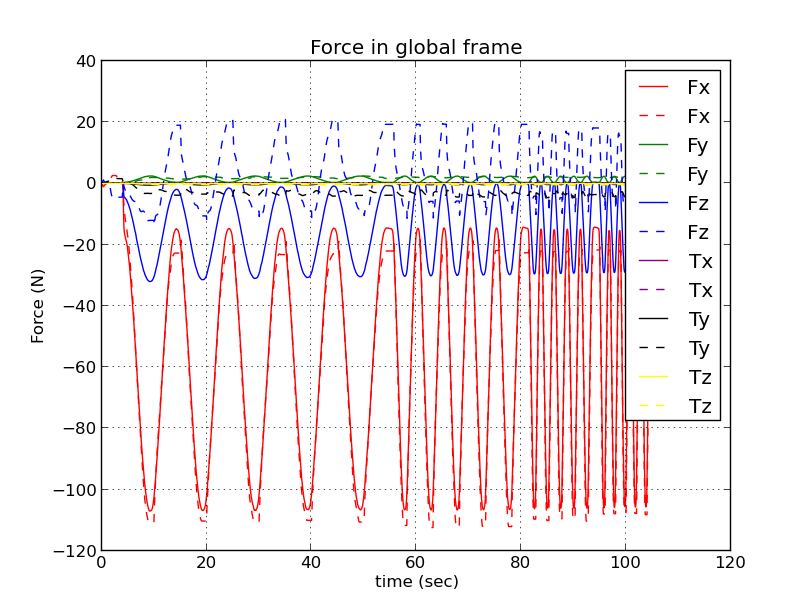
\includegraphics[width = \textwidth ]{fig14} 
    \caption{Using static model}
    \label{fig:static validation}
  \end{subfigure}
  \begin{subfigure}[t]{0.5\textwidth}
    \centering
    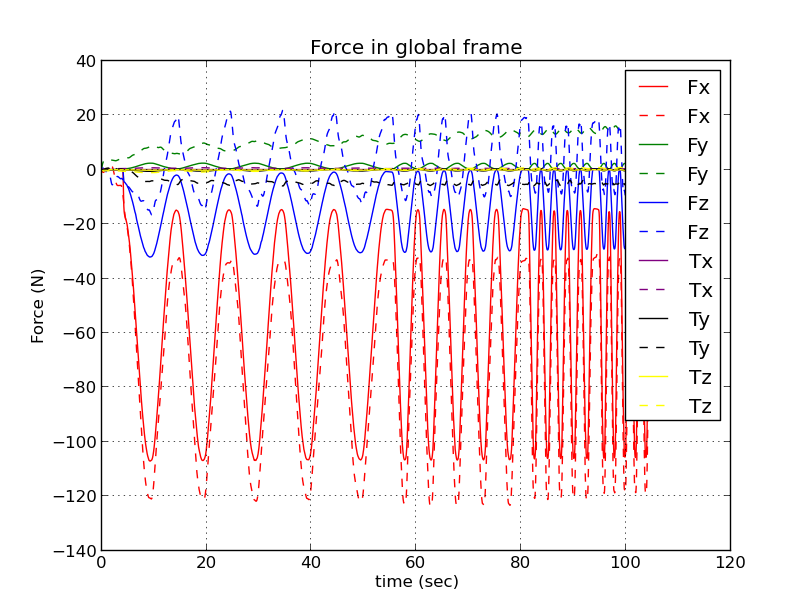
\includegraphics[width = \textwidth ]{fig15}
    \caption{Using Dahl model}
    \label{fig:Dahl validation}
  \end{subfigure}
  \caption{Validation result of estimated force. (- - : estimated output, -- : real output)}
  \label{fig:validation}
\end{figure}

\begin{figure}[H]
  \begin{subfigure}[t]{0.5\textwidth}
    \centering
    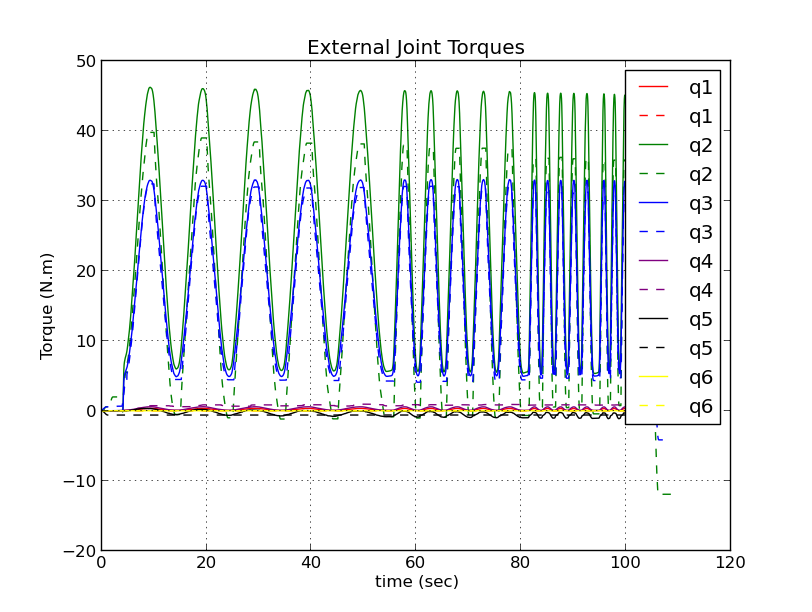
\includegraphics[width = \textwidth ]{fig16} 
    \caption{Using static model}
    \label{fig:static tor}
  \end{subfigure}
  \begin{subfigure}[t]{0.5\textwidth}
    \centering
    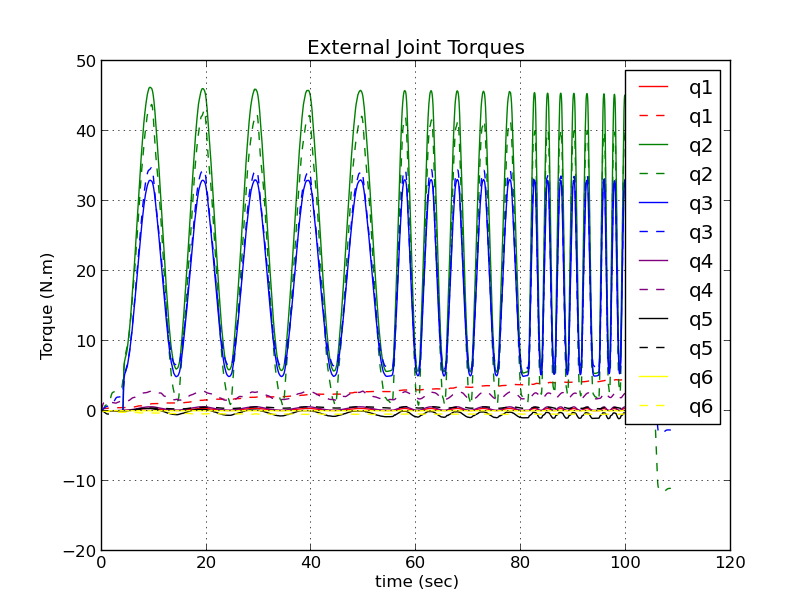
\includegraphics[width = \textwidth ]{fig17}
    \caption{Using Dahl model}
    \label{fig:Dahl tor}
  \end{subfigure}
  \caption{External joint torques estimation of \fref{fig:validation} (- - : estimated output, -- : real output)}
  \label{fig:torque validation}
\end{figure}

In \fref{fig:Dahl tor} it is quite clear that Dahl algorithm gives a good estimation for second and third joint. However, it is bad when estimating the first joint. This is more likely due to two reasons. First, the initial state of $z$ might be incorrect. For every arm position, it is supposed to have specific state of $z$, however as we lack of knowledge of this value, it was only calculated using some basic assumption. The second reason is due to stability of motor currents. Since change of internal state is a function of rate of motor currents, unstable motor currents will drift the value of $z$. However, seeing that the value of first joint seems to be drifted over the time, hence it is more likely that the second reason is the main problem. Due to these problems, it is then decided to leave the Dahl model for the rest of the progress.

On the other hand, the results using coulomb and viscous can be seen in \fref{fig:static validation} and \fref{fig:static tor}. The estimated force in x-axis is quite satisfactory and this is the main force that acting on the robot. However, the force estimation of other axis is not as good as the first one. This is because of the error estimation of external joint torques that leads to the force. The comparison of external joint torques estimation can be seen in \fref{fig:torque validation}. The root mean square error values of estimated contact force and torque using this model are presented in \tref{table:rmse}. On some aspects, especially for torques it has large errors. This is because there is no contact torques introduced, hence the value from force sensor is always near 0.

\begin{table}[H]
    \centering
    \begin{tabular}{| c | c | c | c |}
    \hline
              & RMSE & max-min & RMSE / (max-min)(\%) \\ \hline
    Force x   & 5.231976  & 107.774842  & 4.854543  \\ \hline
    Force y   & 0.942644  & 2.391211    & 39.421205  \\ \hline
    Force z   & 18.686503 & 32.631091   & 57.265945  \\ \hline
    Torque x  & 0.116993  & 0.048434    & 241.550320  \\ \hline
    Torque y  & 3.542738  & 0.879940    & 402.611434  \\ \hline
    Torque z  & 0.350672  & 0.192694    & 181.983440  \\ \hline
    \end{tabular}
    \caption{Root mean square value of estimated contact force using static friction}
    \label{table:rmse}
\end{table}

While it gives a reasonable results for both model, this is partially because the old data was being used for validation, hence it is quite obvious that it will give a good estimation. Validation with new data will be required to really verify the developed model. However, since the methodologies were changed in the middle, these results are not analysed further.


\section{Validation of Two-Stage Experiment Results}

New setups and data that differ from identification data were performed and collected. The algorithm in section \ref{algorithm} was then used to estimate the contact force in offline mode. The results were then compared with the real contact force measured from F/T sensor. 

Three types of contact was performed for the validation. First is static contact force, where the robot was fixed and external force was then introduced to the robot. Second is where the robot was pushing an object in a continuous sinusoidal motion. And the last contact type is where the robot pushed an object with a step function.  

The results could be seen in \fref{fig:force validation 2} for all types of contact. The continuous lines are the measurement from F/T sensor while the strip lines represent the predicted value using the developed algorithm. Results for individual axis can be examined in the appendix (see \fref{fig:appendix static contact} - \fref{fig:appendix step contact}). The root-mean-square from these data are also given in the next table.

\begin{figure}[H]
  \begin{subfigure}[t]{0.5\textwidth}
    \centering
    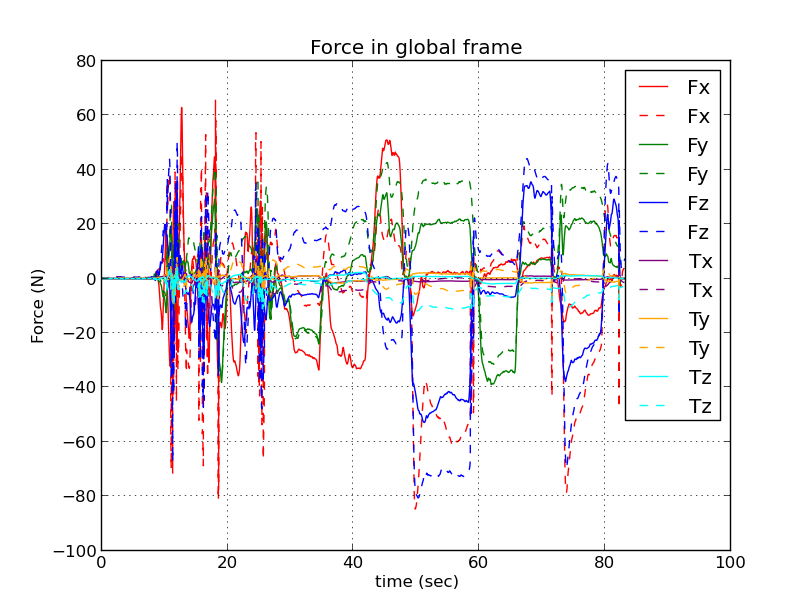
\includegraphics[width = \textwidth ]{Static_contact_force} 
    \caption{Static contact force}
  \end{subfigure}
  \begin{subfigure}[t]{0.5\textwidth}
    \centering
    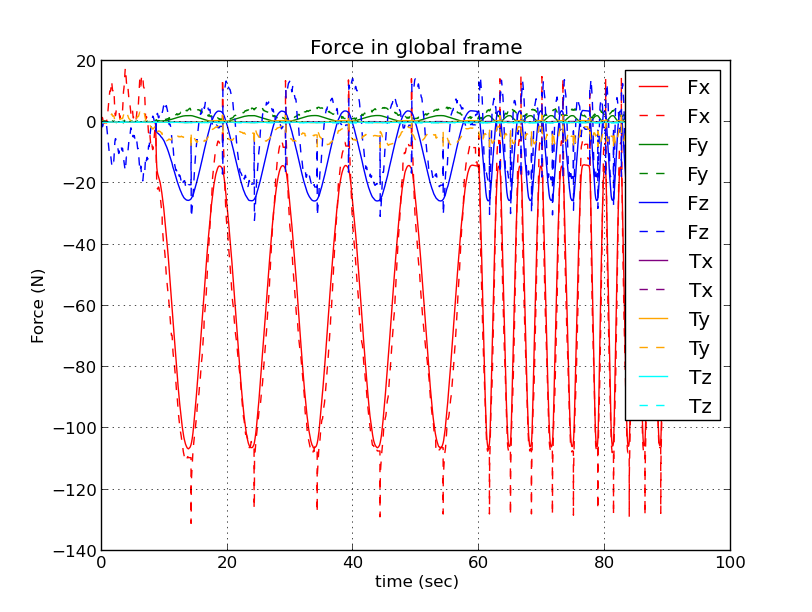
\includegraphics[width = \textwidth ]{Sinusoidal_contact_force}
    \caption{Sinusoidal contact force}
  \end{subfigure}
  \begin{subfigure}[t]{0.5\textwidth}
    \centering
    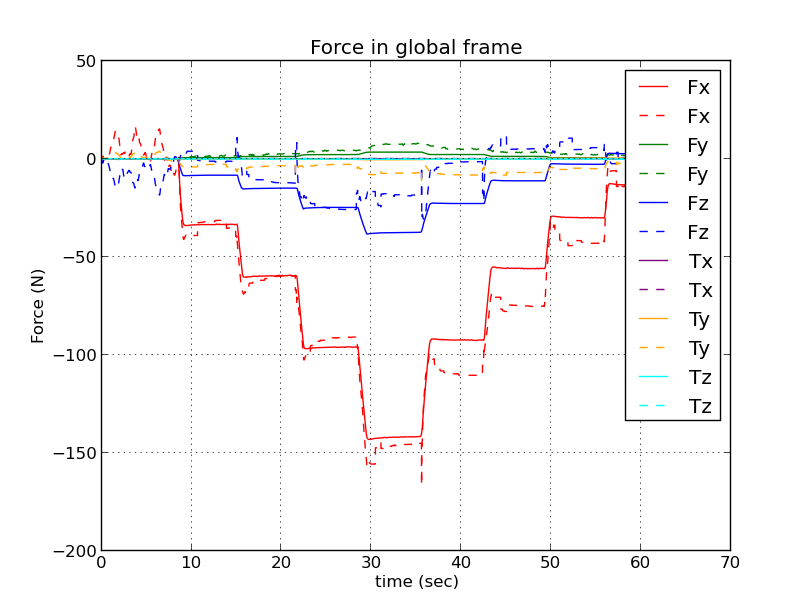
\includegraphics[width = \textwidth ]{Step_contact_force}
    \caption{Step function contact force}
  \end{subfigure}
  \caption{Verification of developed model for various contact type(- - : estimated output, -- : real output)}
  \label{fig:force validation 2}
\end{figure}

\begin{table}[H]
    \centering
    \begin{tabular}{| c | c | c | c |}
    \hline
    \multicolumn{4}{|c|}{Root Mean Square of Various Contact Type} \\\hline
              & static (\%) & sinusoidal (\%)  & step (\%)    \\ \hline
    Force x   &  46.201581  &  7.035855       & 6.812475    \\ \hline
    Force y   &  45.474764  &    79.921285     & 61.432838   \\ \hline
    Force z   &  26.483134  &   33.682928      & 29.129328   \\ \hline
    Torque x  &  146.662725  &  247.210383     & 136.615923  \\ \hline
    Torque y  &  186.067329  &   683.422297     & 532.088055 \\ \hline
    Torque z  &  408.659309  &  90.338212      & 51.192202 \\ \hline
    \end{tabular}
    \caption{Root mean square value for all types of contact}
    \label{table:rmse 2}
\end{table}

From the root mean square value, the estimation gives horrible results for some of the axes. There are  possible explanations for this: 1) The range of external force/torque introduced is small 2) Poor denso gain identification due to the effect of the deadzone and 3) Poor friction identification. For example, torque z in static contact force has a large error that possibly due to the large deadzone of the sixth joint (see \fref{fig:denso gain sixth joint}). On the other hand, torque x and y have a bad estimation during the sinusoidal and step contact force since for this experiment only external force x and z are introduced, thus making the range value is small. In contrast, the model can give a much better estimation for axis with large range of external torque/force. For instance, force x during sinusoidal and step motion has a good estimation of the force. 

Hence, it can be concluded that the model will work better when contact force/torque is large and it will perform poorly for small or no contact force. 
